% !TEX root = ../main.tex
\section{Preprocessing and Validation of Collected Data} \label{sec:preprocessvalidate}
  When collecting data, it is important to preprocess the data before analyzing the data. One of the reasons for preprocessing the data is, for example, to find an outlier in the data. An outlier can impact the data to not show the correct results. For example, when going through the pattern creating time, some of the respondents had used over 10 hours for creating a pattern. The high response time causes noise in the data and is declared as outliers, meaning that the response will be removed from the dataset. Figure \ref{fig:patterncreationtimeoutliner} is a plot of the pattern creation time, using time intervals of 1 seconds and number of occurrences. When time goes up to 30 seconds, the frequency goes down. In a normal situation, a pattern does not take a long time to type. It was therefore decided only to use the patterns being created within 30 seconds, as a pattern time higher do not represent a normal situation. Besides the time used, there was no need for preprocessing the other data and were used as is.  
  
    \begin{figure}[H]
      \centering
      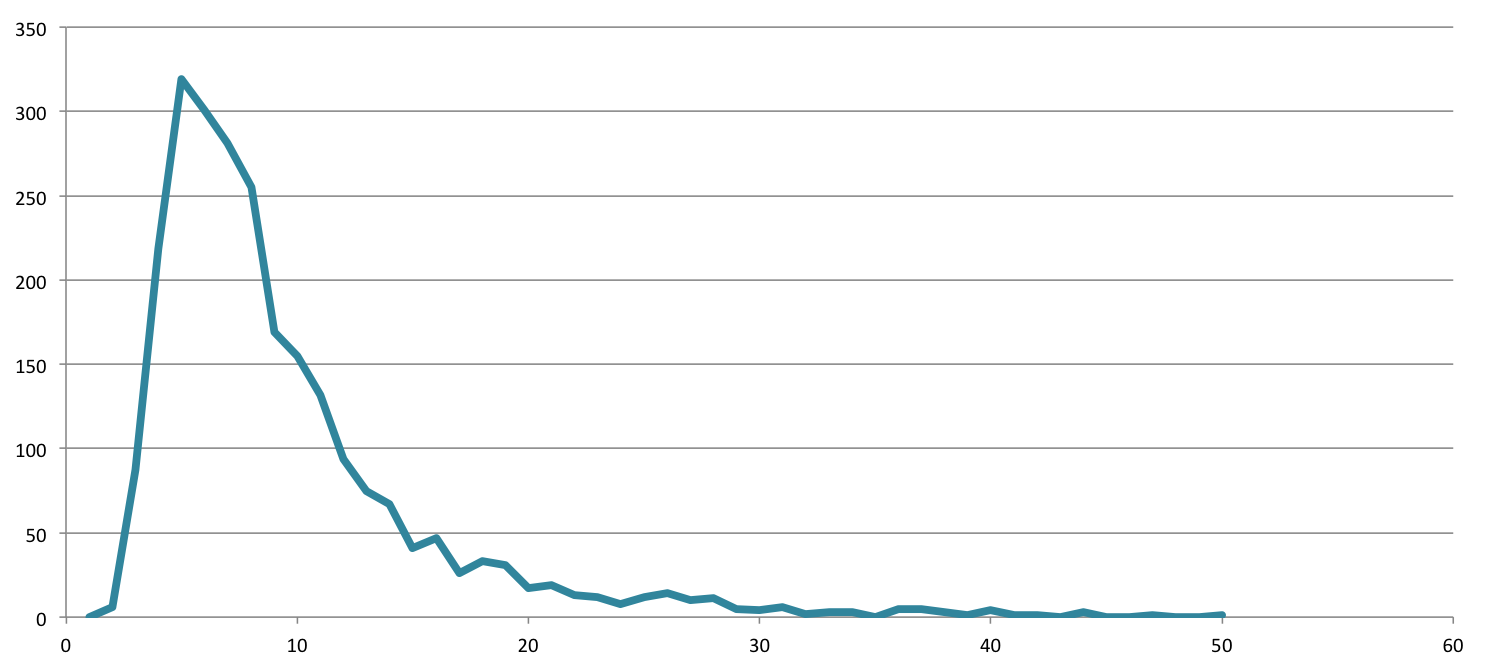
\includegraphics[width=\textwidth]{pics/analysis/limittimeframe.png}
      \caption{Defining max pattern creation time}
      \label{fig:patterncreationtimeoutliner}
    \end{figure}

  It was mentioned that is was used different pattern orders for different respondents. The different orderings were applied to ensure that an ordering was not impacting the choice in patterns. When comparing the time used, the length of the patterns, and visual complexity, there were no significant difference between the patterns created when creating patterns in a different order. Figure \ref{fig:patternOrder} visualises the number of respondents having the different pattern orderings. The specific orders are specified using the numbers 1 to 3 corresponding to patterns created for shopping accounts, smartphones, and banking accounts, respectively. 

		\begin{figure}[H]
      \centering
      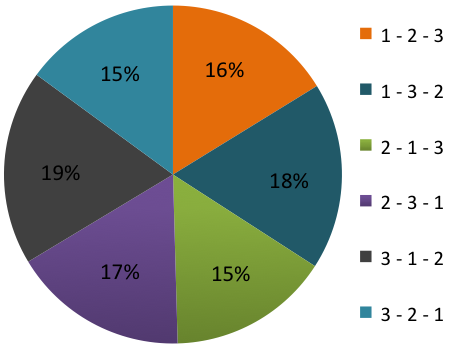
\includegraphics[scale=0.5]{pics/analysis/patternOrder.png}
      \caption{Percentage of times the pattern orders occurred}
      \label{fig:patternOrder}
    \end{figure}
